\section{Introduction}

Fuzzing \cite{li2018fuzzing}, as an automatic testing technique, has become one of the most effective and scalable approaches to exploring vulnerabilities or crashes in commercial off-the-shelf software. Nowadays, it has been widely used by mainstream software companies such as Google \cite{googleossfuzzing} and Microsoft \cite{microfuzzing} to improve their software's reliability and security. The core idea of fuzzing is to feed massive semi-valid inputs to the target program and try to trigger unintended program behaviors (e.g., crash ) by monitoring the system under testing (SUT).

State of the art fuzzing approaches \cite{sutton2007fuzzingbook} \cite{chen2018systematic} could be classified along three dimensions. 

\begin{itemize}
\item \textbf{\textit{Mutation vs. Generation.}} According to ways of generating test cases, fuzzers could be divided into generation-based and mutation-based. Generation-based fuzzers such as Sulley \cite{amini2013sulley} and Peach \cite{eddington2011peach} start without initial seeds. They generate test cases based on specifications of input format and grammar (e.g., protocol session model ) that specify message format and session states. They are more suitable for fuzzing programs that process highly-structured inputs. Mutation-based fuzzers such as AFL\cite{afl}, AutoFuzz \cite{gorbunov2010autofuzz} and SecFuzz\cite{tsankov2012secfuzz}) generate test inputs by mutating pre-provided seeds using various kinds of mutation operators. They could effectively fuzz programs that process with and unstructured data formats.
\item \textbf{\textit{Stdin vs. File vs. Network.}} According to channels of delivering test cases, fuzzing can be classified into stdin fuzzing, file fuzzing, and network(or protocol) fuzzing. Stdin fuzzing provides test cases by standard input and output, file fuzzing provides test cases by opening and reading files, and protocol fuzzing sends and receives test cases based on network communication. 
\item \textbf{\textit{BlackBox vs. WhiteBox vs. GreyBox.}} Depending on the knowledge to the interal of target programs, fuzzers could be classified into BlackBox, WhiteBox and GreyBox fuzzers. Black-box fuzzers \cite{ amini2013sulley} \cite{eddington2011peach} \cite{gascon2015pulsar}) have no knowledge about internals of SUT, and thus relatively less effective. White-box fuzzers usually apply heavy-weight program analysis such as taint-analysis \cite{ganesh2009taint-white} \cite{wang2010taintscope} or symbolic execution \cite{stephens2016driller}  \cite{godefroid2012sage} to improve effectiveness, but may suffer from scalability problems. GreyBox fuzzers such as AFL \cite{afl} and its variations (e.g. AFLFast \cite{bohme2016aflfast}, FairFuzz \cite{fairfuzz}, AFLGo \cite{bohme2017aflgo}, CollAFL \cite{gancollafl}, etc.), LibFuzzer \cite{infrastructure2017libfuzzer} are in between. They apply light-weight program analysis and trivial instrumentation to collect coverage information of the SUT as feedback. Then these feedbacks are used to drive fuzzing. GreyBox fuzzers improve fuzzing efficiency without significantly sacrificing execution speed and scalability.
\end{itemize}

State-of-the-art feedback-driven and mutation-based grey box fuzzing tools include AFL \cite{afl} and its variations (e.g., AFLFast \cite{bohme2016aflfast}, FairFuzz \cite{fairfuzz}, AFLGo \cite{bohme2017aflgo}, CollAFL \cite{gancollafl}, etc.), LibFuzzer \cite{infrastructure2017libfuzzer}, honggfuzz\cite{swiecki2016honggfuzz}, etc. They have proved extremely effective and promising in detecting vulnerabilities because of the improved code coverage. 

%related work
However, none of existing grey box fuzzing tool could explore entire search space exhaustively for real-world programs in practice, especially when time and computation resources are limited. To make a fuzzer more powerful, many improvement works have been done, which could be categorized into three directions:

\begin{itemize}
\item \textbf{Effectiveness.} It aims to improve meta-abilities of fuzzers to bypass obstacles and trigger vulnerabilities. It contains aspects such as (1) feedback accuracy \cite{gancollafl} and granularity \cite{li2017steelix}; (2) mutation strategies ( i.e. where and what to mutate) \cite{rawat2017vuzzer} \cite{peng2018t} \cite{wang2010taintscope} \cite{chen2013angora};  (3) sensitiveness to security violation \cite{serebryany2012addresssanitizer} \cite{stepanov2015memorysanitizer} and so on.
\item  \textbf{Efficiency.} It aims to improve performane on maximizing code coverage, and improve probability of triggering vulnerabilities. It contains aspects like (1) providing high quality and diversity of intial seeds \cite{wang2017skyfire} \cite{godefroid2017learn} \cite{nichols2017faster} \cite{lv2018smartseed}; (2) improving execution speed by prioritizing faster seed, using new primitives \cite{xu2017designing} and utilizing system fork mechanism and hardware features (e.g Intel-PT) \cite{schumilo2017kafl} \cite{zhang2018ptfuzz}; (3) balancing fuzzing energy distribution like low-frequence and untouched path deserves more energy \cite{bohme2016aflfast} \cite{rawat2017vuzzer} \cite{gancollafl}. 
\item \textbf{Guidance.} It aims to make fuzzing be directed effectively for some specific goals. AFLGo \cite{bohme2017aflgo} directs fuzzing to reach some specific location (i.e., line of code) as soon as possible. SlowFuzz \cite{petsios2017slowfuzz} directs fuzzing to trigger specific kinds of bugs (i.e., algorithmic complexity vulnerabilities).
\end{itemize}

In this paper, we focus on AFL based grey box fuzzing. Two new insights about existing AFL based fuzzers' energy distribution are gained during the process of using these fuzzers.

%\textbf{Insight 1: } Existing energy distribution strategy discriminate against time-consuming (TC) paths, which are usually paths containing long loops or complex algorithm.  TC paths are ignored with significant probability and given little energy even if not ignored. This discrimination makes it difficult to detect vulnerabilities buried in TC paths, such as bugs behind long loops.  Thus, TC  paths should be given more opportunities at the right time to balance the possibility of discovering vulnerabilities in TC paths.

%The growth of the path follows the same pattern.  In the beginning, it increases quickly, and the growth rate gradually becomes flat. After a certain period, the path growth becomes more and more difficult. There are two reasons for this phenomenon. The natural reason is that the discovery problem of the new path is a Coupon Collector’s Problem(CCP), After finding $i-1$ new paths, the probability of finding the new path of the $i$th is $P_{i}= (N-i+1)/N$, where $N$ is the total paths. 

%\begin{figure*}[t]
%    \centering
%    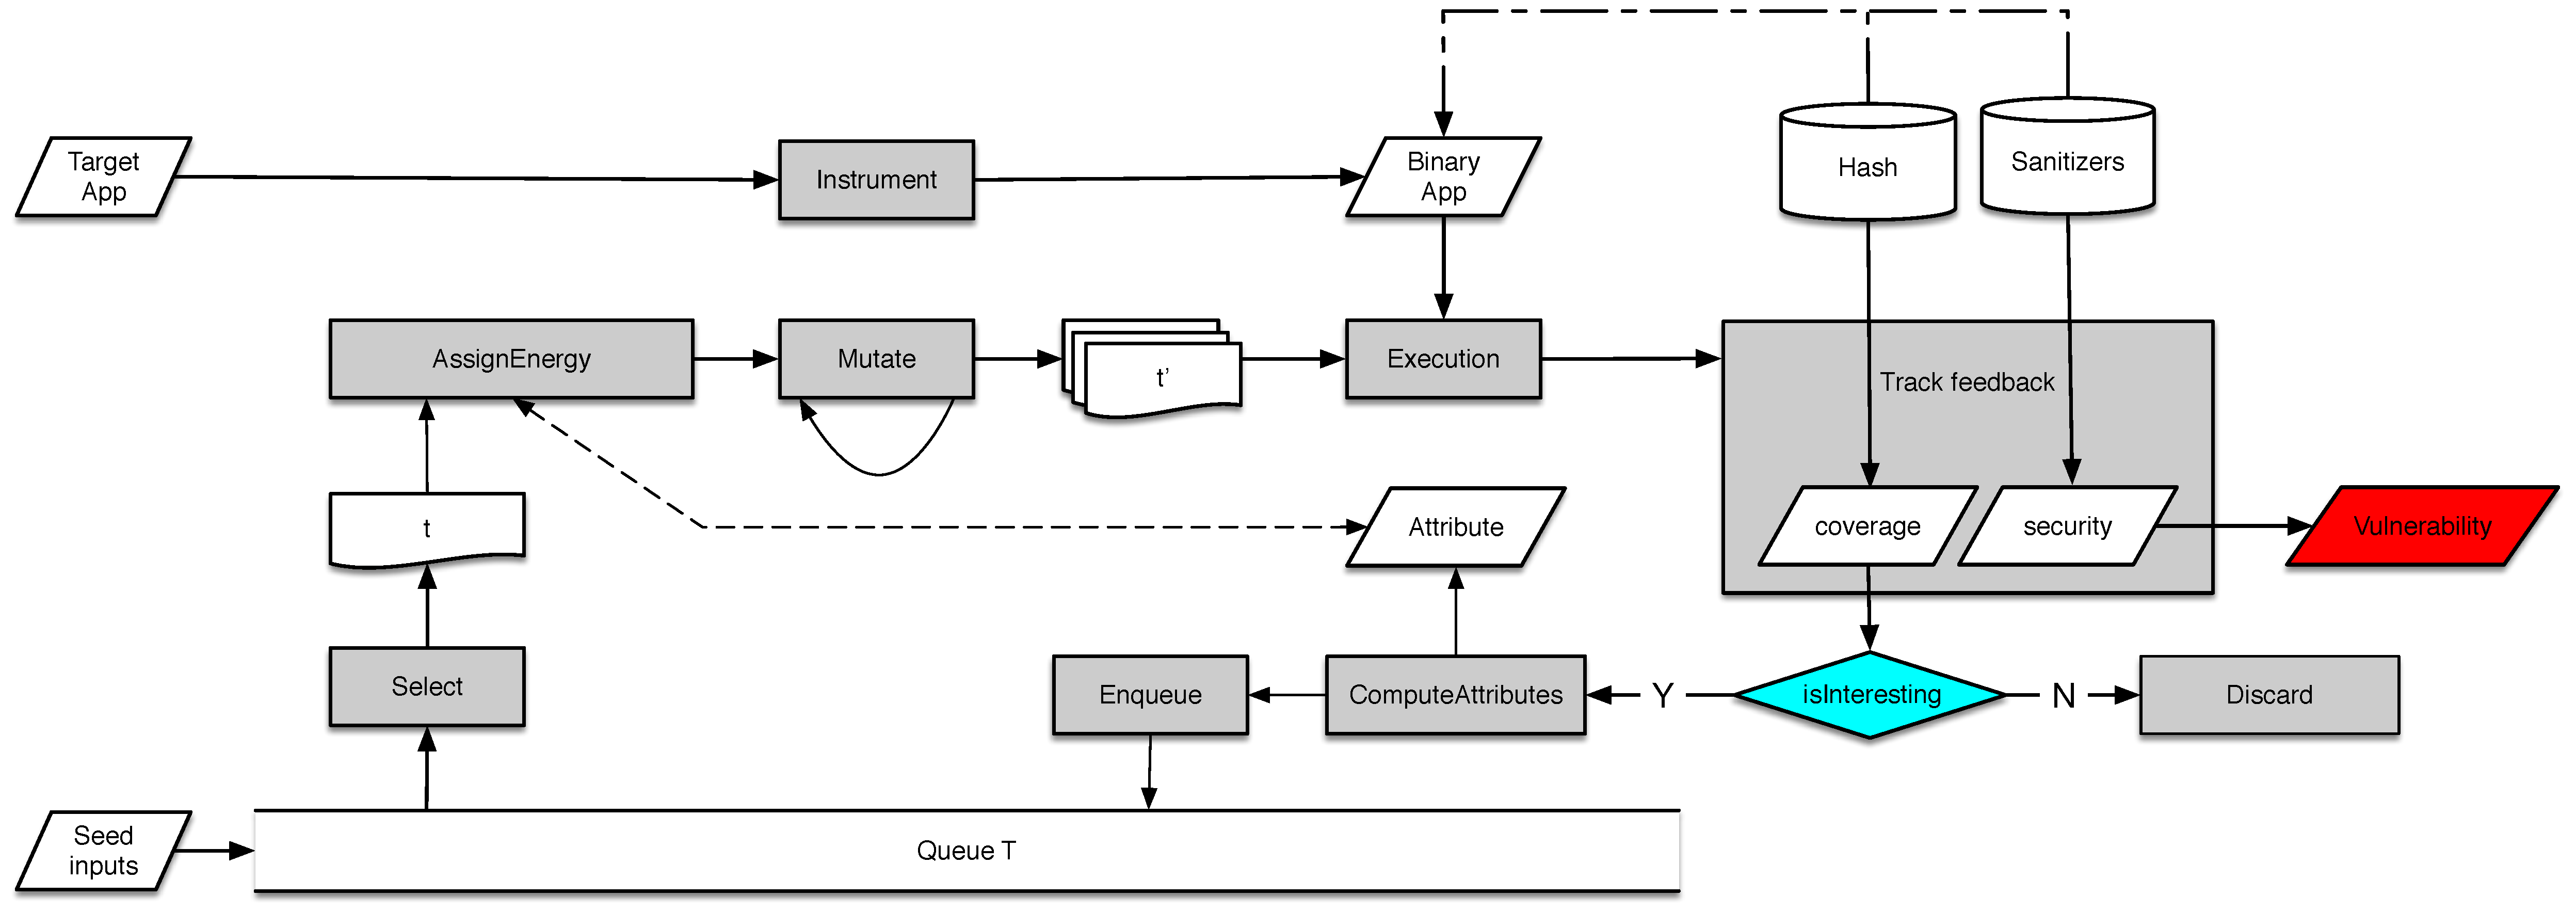
\includegraphics[width=5.5in]{pic/AFL.eps}
%    \caption{The general workflow of AFL  based grey box fuzzing}
%    \label{AFL}
%\end{figure*}
\textbf{Insight 1:} One crucial factor of vulnerability discovery is whether regions that vulnerabilities reside are explored. If vulnerability-residing regions are prioritized and strengthened to be fuzzed, then vulnerabilities could be detected faster and more bugs may be found during same period of time. Existing improvements on guidance are trying to direct fuzzing to reach a specific  location (i.e., the line of code) given in advance, rather than towards promising regions that are more likely for a vulnerability to reside. There are some understanding that sensitive regions(i.e., regions which contain more memory or string operators), complex regions (i.e. code regions with high complexity), deep regions, and rare-reach regions of a program may have more chance to be vulnerable. Thus, guided fuzzing through optimized energy distribution towards these promising vulnerable regions could improve fuzzers' efficiency and detect more bugs. 

\textbf{Insight 2:} Existing energy distribution strategies only tune the mutation number, and randomly select mutation operators.
Empirical studies have shown that coarse-grained mutators (e.g., extra mutators) have better ability to generate diversity test cases, which is helpful for path growth, while fine-grained mutators tend to perform better in exploring nearby execution paths.
Therefore, a better strategy is to adjust the proportion of different granularity mutation operators over time. If certain kinds of mutators perform better, we increase the ratio of these mutators, and vice versa.

\textbf{Key Observation:} Both insight 1 and insight 2 imply that energy distribution matters in greybox fuzzing.

\textbf{Problem Statement:} How to leverage the two insights to improve existing energy distribution strategies and improve the efficiency of AFL based greybox fuzzers?

\textbf{Our Work:} We leverage the two new insights to improve existing AFL's fuzzing energy distribution in a principled way. We direct fuzzers to stress fuzzing toward regions that are more likely for a vulnerability to reside based on static semantic metrics of target program. More specifically, four kinds of promising vulnerable regions (i.e., sensitive, cpmplex, deep and rare-reach regions) are evaluated. And a granularity-aware scheduling of different mutation operators is proposed. The ratio of certain kinds of mutation operators is increased gradually, if they have better ability to trigger new paths. All improvements are integrated and implemented into an newly developed open source fuzzing tool named TAFL. Large-scale experimental evaluations have shown effectiveness of each improvement and the integration. Furthermore, TAFL helps us find five unknown bugs and one new CVE in Libtasn1-4.13\cite{bugs}.

In summary, contributions of our work are as follows:

\begin{itemize}
    \item \textbf{Insights.} We provide two new insights into the energy distribution of AFL based greybox fuzzing.
    
    \item \textbf{Improvements.} We improve the energy distribution strategy in a principled way by leveraging two new insights. More specifically, we improve guidance by directing fuzzing toward four kinds of promising vulnerable regions, and scheduling of different kinds of mutation operators.
    
    \item \textbf{Tool.} We implement and integrate our improvements into a new fuzzing tool named TAFL, which could be accessible from: 
              \url{https://sites.google.com/view/tafl/tool}.
    
    \item  \textbf{Vulnerabilities.} We perform large-scale experimental evaluations to show effectiveness of each improvement and performance of integration. Furthermore, TAFL helps us to find five unknown bugs and one new CVE in Libtasn1-4.13.

\end{itemize}

The remainder of this article is structured as follows: Section \ref{background} is the introduction of American Fuzz Lop (AFL). Section \ref{newinsight} explains our new insights of existing AFL's energy distribution.  Section \ref{approach} gives details of the improvements method by leveraging two insights. Section \ref{impl} describes implementation details. Section \ref{experiment} is the experimental evaluation of each improvement and performance of integration. Section \ref{relatedwork} states related works. Finally, we conclude our work in Section \ref{conclusion}. 







